%\chapter[Основные принципы, правила и методы конструирования деталей и\\ функциональных устройств ОЭП]{Основные принципы, правила и методы конструирования деталей и функциональных устройств ОЭП}

\section{Принципы конструирования деталей}

\begin{flushleft}
	\textbf{Общие аспекты конструирования деталей}
\end{flushleft}

Рассмотрим кратко некоторые общие, а также специфические вопросы конструирования деталей. 

\textit{Детали} являются простейшими объектами конструирования и представляют собой неделимые однородные тела, состоящие из элементов формы (геометрических поверхностей тел) и материала.

В каждой детали различают следующие структурные элементы (поверхности): рабочие (активные), базовые, соединительные (свободные) и технологические.

\textit{Рабочие элементы} (РЭ -- их называют также активными или исполнительными поверхностями) непосредственно выполняют заданные функции детали. Например, РЭ являются: сферические поверхности линзы (рис.~\ref{pic:4det}~а); эвольвентная поверхность зубчатого венца колеса (рис.~\ref{pic:4det}~б); плоская и цилиндрическая поверхности гнезда оправы линзы (рис.~\ref{pic:4det}~в). Эти поверхности, как правило, тщательно обрабатываются, и к ним предъявляются высокие требования: точность расположения, погрешность формы, чистота поверхности, размеры.

\textit{Базовые элементы} (БЭ) обеспечивают координацию детали (т. е. координацию ее РЭ) относительно других деталей и представляют собой поверхности, по которым деталь сопрягается (соединяется) с базовой деталью (рис.~\ref{pic:4det}). Данные поверхности изготавливаются также весьма тщательно.

\textit{Соединительные элементы} (СЭ -- их называют часто свободными) служат для обеспечения материальной связи между рабочими и базовыми элементами (рис.~\ref{pic:4det}). К СЭ не предъявляются высокие требования по тщательности и точности изготовления (за исключением требований к чистоте поверхностей, когда это обусловлено эстетическими показателями качества детали).

\begin{figure}[H]
	\caption{Структурные элементы деталей}
	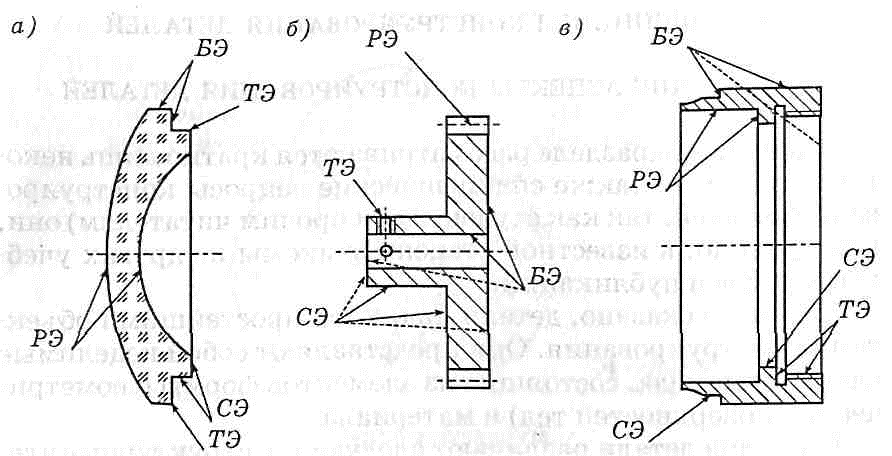
\includegraphics[width=1\textwidth]{4det.png}
	\label{pic:4det}
\end{figure}

\textit{Технологические элементы} (ТЭ) служат для обеспечения технологического процесса изготовления и последующей сборки детали (например, фаски, галтели, выточки, центровые отверстия в валиках). Для линзы (рис.~\ref{pic:4det}~а) ТЭ являются фаски, которые устраняют выколки, появляющиеся на кромках при ее шлифовке; для зубчатого колеса (рис.~\ref{pic:4det}~б) ТЭ является резьбовое отверстие под стопорный винт для фиксации зубчатого колеса на валике при рассверливании отверстия под штифт; в оправе линзы (рис.~\ref{pic:4det}~в) ТЭ является резьба (и канавка для выхода резьбы) для закрепления оправы (с линзой) в центрировочном патроне для результативной обработки ее базовых поверхностей в размер.

Следует отметить, что одни и те же поверхности (части поверхностей) могут выполнять роль РЭ, БЭ и СЭ. Наиболее благоприятным считается вариант, когда в конструкции удается объединить РЭ и БЭ, минимизировать СЭ.

Конструирование детали заключается в выборе материала, формы ее поверхностей и определения ее размеров. Кроме этого, конструктор должен указать допустимые отклонения характеристик материала, погрешности изготовления размеров и форм, тип покрытий, вид обработки, технические и технологические условия и требования (например, азотирование, просветление, старение).

Выбор материала производится исходя из функционального назначения детали, условий ее эксплуатации, рациональной технологии изготовления, стоимости и дефицитности материала, требований эргономики и эстетики.

Конструктор руководствуется при этом номенклатурой и физико-механическими свойствами конструкционных материалов (табл.~\ref{tab:prop}).

\begin{table}[h]
	\caption{Физико-механические и технологические свойства материалов}
	\label{tab:prop}
	\begin{tabular}{|c|c|} \hline 
		Свойства & Характеристики \\ \hline
		\multirow{5}{*}{Механические} & Плотность\\ 
		& Упругость \\ 
		& Твердость \\
		& Износотойкость \\
		& Прочность\\ \hline
		\multirow{5}{*}{Тепловые} & Коэффициент линейного расширения\\
		& Теплопроводность \\
		& Теплоемкость \\
		& Термооптические постоянные \\
		& Термостойкость \\ \hline
        \multirow{4}{*}{Химические, коррозионные} & Налетоопасность \\
        & Радиационная устойчивость \\
        & Коррозионная стойкость \\
        & Водопоглощаемость (влагостойкость)\\ \hline
        \multirow{3}{*}{Электромагнитные} & Удельное электрическое сопротивление \\
        & Магнитная проницаемость \\
        & Пробивная электрическая прочность\\ \hline
        \multirow{4}{*}{Фрикционные} & Коэффициент трения скольжения \\
        & Коэффициент трения качения \\
        & Коэффициент сцепления \\ \hline
        \multirow{4}{*}{Технологические}  & Пластичность \\
        & Свариваемость \\
        & Прессуемость \\
        & Трудоемкость обработки \\ \hline
	\end{tabular}
\end{table}

Например, если конструируется линза, то ее материал должен быть прозрачным для рабочего диапазона длин волн света. Если линза будет эксплуатироваться в условиях тропического или морского климата, необходимо выбрать материал, стойкий к воздействию влаги, грибков, соли и других вредных факторов. Исходя из условия минимизации массы, возможности получения линзы литьем, она могла бы быть изготовлена из органического стекла (если это не влияет на другие показатели качества детали).

Естественно, что характеристики используемого материала должны обеспечить необходимую точность размеров, форм и шероховатость (чистоту) поверхностей детали при ее изготовлении, а также сохранение их стабильными в процессе длительной эксплуатации при воздействии различных факторов.

Технологичными считаются материалы, которые легко обрабатываются резанием, шлифуются, штампуются, прессуются, свариваются, спекаются, имеют хорошие литейные свойства. Общей современной тенденцией являются использование таких материалов, из которых можно изготавливать детали производительными методами (например, литьем под давлением, штамповкой, прессованием), а также широкое применение пластмасс.

При выборе материала деталей, взаимодействующих с человеком как непосредственно, так и косвенно, учитываются эргономические показатели: гигиенические, антропометрические и психофизиологические (уровень шума, амплитуда и частота вибраций, температура, возможность получения оптимальной формы, усилия, контраст, класс исполнения, степень утилизации). Например, такой перспективный для изготовления космических зеркал материал, как бериллий, обладающий для этого рядом очень хороших характеристик, является весьма токсичным при обработке, что ограничивает его использование.

Свойство материала обуславливает также достижение соответствия формы внешних деталей их назначению, качество и совершенство отделки, возможность нанесения декоративных покрытий и другие эстетические показатели.

В общем случае решение задачи по выбору материала детали является многовариантным, так как требования к точности, надежности, массе, прочности, жесткости, экономичности, эстетичности и др. вступают в противоречие друг с другом, которое приходится преодолевать, оптимизируя выбор материала с помощью ранжирования значимости показателей качества детали и свойств материала. Весьма часто выбор материала производится с помощью расчета необходимых значений некоторых его характеристик по требуемым показателям качества (например, марок и оптических констант стекла по допустимым аберрациям системы, модуля упругости материала валика по его допустимым деформациям, коэффициента линейного расширения материала по допустимым изменениям размеров детали при изменении температуры).

Конструктор должен постоянно следить за появлением новых материалов, а также пытаться использовать нетрадиционные (для ответственных деталей) материалы, которые благодаря своим свойствам могут повысить показатели качества проектируемого изделия.

Выбор формы ограничивающих деталь поверхностей осуществляют исходя из их структуры (функционального назначения), технологичности, эстетических и эргономических требований, конструктивной целесообразности. Форма рабочих элементов типовых деталей часто бывает вполне определенной. Примерами могут служить сферические поверхности линз, плоские поверхности преломляющих и отражающих граней призм, эвольвентные поверхности зубьев зубчатого колеса, спиральный профиль кулачка.

Рабочие элементы оригинальных деталей выполняют в виде специальных поверхностей, например параболическими, эллиптическими, торическими. Форма базовых, свободных и технологических элементов обычно представляет собой типовые поверхности -- плоскость, цилиндр, конус, сферу -- для оптических. Более технологичными являются типовые поверхности, получаемые при обработке деталей на универсальном оборудовании типовым инструментом.

Параметры формы могут быть получены эвристически, расчетным путем, исходя из условий стандартизации и унификации, технологических возможностей производства (например, радиусы кривизны сферических поверхностей линз определяют из аберрационного расчета и ГОСТов на них, угол конуса конической или дугообразной поверхности центрового отверстия детали назначают исходя из типа детали, ее массы, требований к точности обработки и ГОСТ~14034-74).

Определение размеров детали производится с учетом большого числа факторов, среди которых следует выделить функциональную точность, параметрическую надежность, жесткость, компактность, эстетичность и эргономичность, технологичность, требования стандартизации и унификации, массу и используемые материалы. Конструктор, руководствуясь вышеперечисленными факторами, выбирает или рассчитывает необходимые размеры структурных элементов детали.

В наиболее ответственных случаях детали подвергаются тщательному расчету (а иногда и экспериментальным исследованиям) по математическим моделям, связывающим ее размеры (и параметры формы) с требуемыми показателями качества, компоновкой, условиями эксплуатации, производства и другими ограничениями. Как правило, это детали, определяющие точность функционирования, качество создаваемого изображения, испытывающие значительные статические, динамические, тепловые нагрузки (например, детали астрономических, военных, космических приборов).

Для оптических деталей подобными расчетами (например, габаритно-аберрационным) определяют размеры и расположение рабочих элементов. Весьма важный аспект конструирования детали -- это обеспечение технологичности ее конструкции (ГОСТ~14.204-73), значимой характеристикой которой является трудоемкость изготовления и в дальнейшем сборки детали.

Трудоемкость изготовления детали зависит от рациональности выбранного материала и оптимальности ее форм и размеров для условий современного производства. 

При конструировании деталей конструктор должен определить способ термообработки, тип покрытий и смазочный материал, которые оказывают существенное влияние на показатели их назначения и особенно надежности.

Благодаря термообработке (закалке, отжигу, старению) улучшаются, например, характеристики прочности и твердости, износостойкости, снижаются остаточные напряжения (вызывающие их деформацию во времени), появляется возможность получения более точных поверхностей в деталях.

Покрытия деталей позволяют защитить их от коррозии (налетоопасности, пятнаемости), улучшить их внешний вид, уменьшить износостойкость, изменить некоторые характеристики (например, теплопроводность, электрическое сопротивление, коэффициент отражения).

Особенно широко применяются покрытия оптических деталей: просветляющие, зеркальные, поляризующие, токопроводящие, покрытия-фильтры, защитные.
Смазочные материалы, (замазки) предназначены для уменьшения трения и износа подвижных деталей, защиты от коррозии, герметизации и влаго- и пылезащиты.

Вопросы термообработки, покрытий, смазки деталей точных приборов изложены в соответствующих справочниках, ГОСТах и специальной литературе.

\begin{flushleft}
\textbf{Принцип совместной обработки рабочих и базовых элементов детали}
\end{flushleft}

Этот принцип заключается в предпочтительности конструкции детали, позволяющей осуществлять совместную технологическую обработку (за одну установку) ее рабочих и базовых элементов, так как в этом случае точность их взаимного расположения будет выше.

На рис.~\ref{pic:4oprava} изображены варианты упрощенной конструкции оправы линз объектива, в одном из которых оба рабочих элемента (РЭ$ _1 $, РЭ$ _2 $) не могут быть обработаны совместно с базовым элементом (рис.~\ref{pic:4oprava}~а), а в другом такая возможность существует (рис.~\ref{pic:4oprava}~б). В первом случае погрешность расположения РЭ$ _2 $ относительно РЭ$ _1 $ и БЭ будет больше, а следовательно, хуже центрировка линз и точность выдерживания воздушного промежутка, чем во втором варианте. Обусловлено это тем, что при перестановке (технологическом перебазировании) оправы в патроне станка возникают погрешности взаимного расположения ее РЭ и БЭ, обусловленные изменением технологической и измерительных баз.

\begin{figure}[H]
	\caption{Конструкции оправы}
	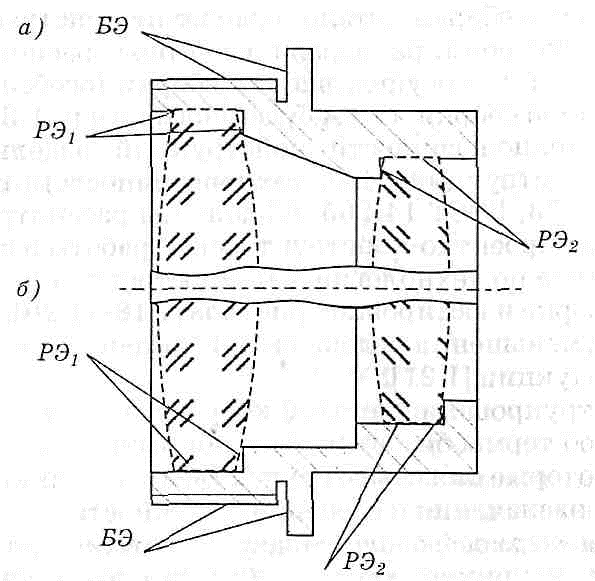
\includegraphics[width=0.4\textwidth]{4oprava.png}
	\label{pic:4oprava}
\end{figure}

\begin{flushleft}
\textbf{Принцип точностной технологичности деталей}
\end{flushleft}

Этот принцип заключается в учете экономических факторов при назначении допусков на характеристики материала детали и на погрешности ее изготовления.

Конструктор должен помнить, что от допусков на деталь в существенной степени зависит ее стоимость. Назначение высоких (жестких) допусков на погрешности изготовления деталей приводит к существенному их удорожанию, поэтому такие допуски должны быть обоснованы другими факторами, связанными, например, с затратами на сборку, точностью функционирования всего прибора. Также,  чем выше качество используемого материала, тем она дороже. Например, стоимость оптического стекла первой категории класса А по показателю преломления и средней дисперсии в несколько раз больше, чем стекло той же марки пятой категории класса Г, а его стоимость с учетом всех показателей качества может отличаться на порядок.

\section{Принципы конструирования соединений}

\textit{Соединением деталей} в конструкторском смысле (как элемента конструкции) называют конструкцию элементарной сборочной единицы, которая состоит из двух или нескольких деталей, находящихся в непосредственном контакте (сопряжении) друг с другом. 

\textit{Соединением деталей} в технологическом смысле (как сборочную операцию) называют сопряжение деталей путем их сочленения, свинчивания, развальцовки, сварки

Соединяемые детали образуют контактные пары, которые классифицируют как: подвижные и неподвижные; замыкающиеся формой, силой и креплением; сопрягающиеся (контактирующие) по поверхности, по линии и по точке.

В соединении различают базовую и рабочую (присоединяемую) детали, а также базовые (БЭС) и рабочие (РЭС) элементы (поверхности) соединения.

На рис.~\ref{pic:4elements} показано соединение линзы (рабочая присоединяемая деталь~1) с оправой~2 (базовая деталь) с помощью резьбового кольца~3, которое является в соединении вспомогательной деталью, осуществляющей силовое замыкание линзы на торцевую посадочную поверхность оправы.

\begin{figure}[H]
	\caption{Элементы, соединения, деталей}
	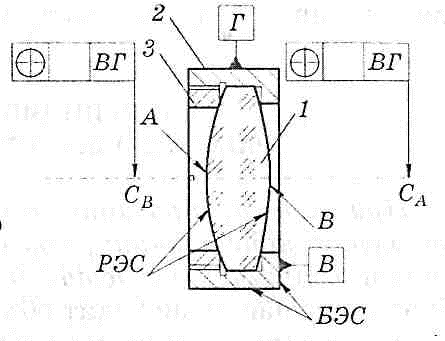
\includegraphics[width=0.6\textwidth]{4elements.png}
	\label{pic:4elements}
\end{figure}

Показатели качества соединений подразделяются: на эксплуатационные (точность, надежность, износостойкость, несущая способность); конструктивные (габаритные размеры, масса, компактность); технологические (технологичность сборки, юстировки и контроля).

Конструируя соединения, в первую очередь стараются достичь их точности (характеризуемой погрешностью расположения РЭС относительно БЭС, рис.~\ref{pic:4elements}), надежности и технологичности.

Рассмотрим принципы конструирования соединений, позволяющие обеспечить эти показатели, основанные на общих правилах и законах наложения материальных связей деталей друг на друга в соединении.

\begin{flushleft}
\textbf{Принцип совмещения рабочих элементов в соединении}
\end{flushleft}

При конструировании соединений предпочтительной является конструкция, позволяющая осуществлять контакт сопрягаемых деталей по их рабочим элементам. В этом случае происходит объединение рабочего и базового элементов присоединяемой детали, уменьшается размерная цепь и повышается точность расположения РЭС относительно БЭС.

На рис.~\ref{pic:4mirror} изображена конструкция соединения зеркала 1 с кронштейном 2. Конструкция, изображенная на рис.~\ref{pic:4mirror}~б, позволяет точнее ориентировать отражающую поверхность зеркала (РЭС) относительно основания кронштейна (БЭС) и не требует жесткого допуска на клиновидность зеркала по сравнению с конструкцией, изображенной на рис.~\ref{pic:4mirror}~а.

\begin{figure}[H]
	\caption{Соединение зеркала с оправой}
	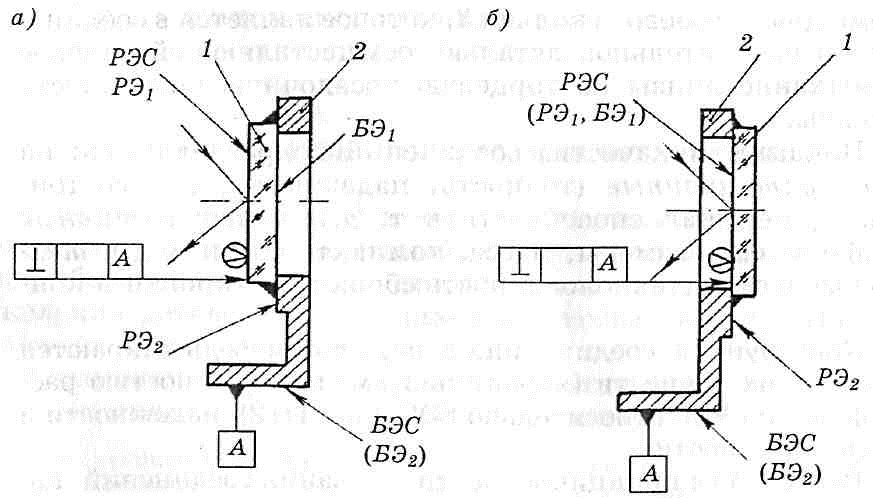
\includegraphics[width=0.7\textwidth]{4mirror.png}
	\label{pic:4mirror}
\end{figure}

\begin{flushleft}
\textbf{Принцип отсутствия избыточного базирования в соединении деталей -- статическая определенность соединений}
\end{flushleft}

Придание материальным телам определенного и строго фиксированного положения в пространстве называют базированием. При базировании происходит отнятие лишних степеней свободы присоединяемой детали относительно базовой в их соединении.

Базирование называют избыточным, когда лишние степени свободы присоединяемой детали отняты более одного раза, т.е. когда для отнятия лишней степени свободы наложена более чем одна связь. Соотношение между оставшимися степенями свободы $n$ и числом наложенных связей $ m $ должно быть $ n+m = 6 $.

В некоторых случаях нарушение принципа можно видеть невооруженным глазом~-- по дублированию сопряжений деталей (базовых элементов), отнимающих одни и те же степени свободы у присоединяемой детали относительно базовой (рис.~\ref{pic:4double}~а).

Устранить неопределенность базирования можно изменив конструкцию сопряжения деталей (рис.~\ref{pic:4double}~б). 

\begin{figure}[H]
	\caption{Дублирование в сопряжении деталей}
	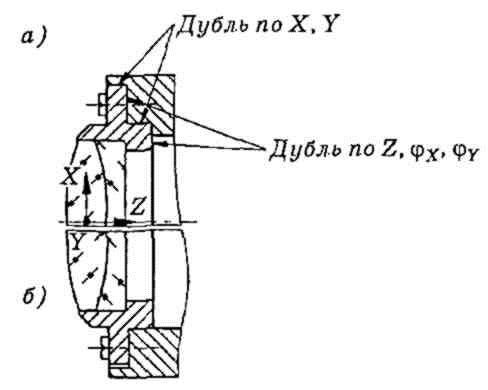
\includegraphics[width=0.6\textwidth]{4double.png}
	\label{pic:4double}
\end{figure}

\begin{flushleft}
\textbf{Принцип геометрической определенности контакта пар в соединении}
\end{flushleft}

Этот принцип заключается в определенности положения и формы, контакта сопрягаемых поверхностей деталей. Реальные поверхности деталей имеют макро- и микропогрешности формы поверхностей. В результате детали контактируют друг с другом не по линиям и поверхностям, а по пятнам (площадкам) неопределенной формы, размеры и положения которых в сопряжении также неопределенны.

Эта неопределенность снижает точность расположения присоединяемой детали и несущую способность базовой детали. Наибольшее влияние на точность оказывает неопределенность расположения пятен контакта.

На рис.~\ref{pic:4connect}~а изображено соединение зеркала~1 с оправой~2 с помощью трех угольников. Из-за погрешностей формы сопрягаемых поверхностей зеркала и оправы их контакт будет происходить не по плоскости, а по трем площадкам 3, расположение и форма которых могут быть произвольными в пределах сопрягаемых поверхностей. В результате возникает объемная деформация зеркала под действием сил $ F $ со стороны угольников и реакции $ R $ со стороны оправы, приводящая к порче качества изображения.

Соединение, изображенное на рис.~\ref{pic:4connect}~б, обладает определенностью расположения площадок контакта благодаря специальным выборкам (либо прокладкам) на оправе. Здесь возникает только контактная деформация зеркала в пределах контактирующих зон, не приводящая к ухудшению качества изображения.

\begin{figure}[H]
	\caption{Сопряжение зеркала с оправой}
	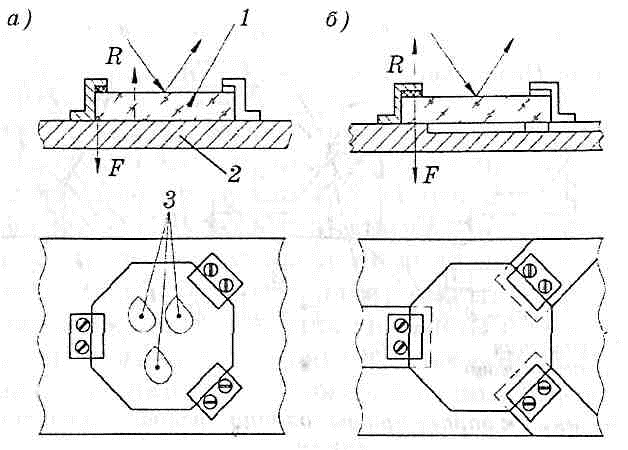
\includegraphics[width=0.85\textwidth]{4connect.png}
	\label{pic:4connect}
\end{figure}

\begin{flushleft}
\textbf{Принцип силового замыкания}
\end{flushleft}

Силовое замыкание соединений следует осуществлять так, чтобы линия действия замыкающей силы проходила через зону (площадку) контакта сопрягаемых поверхностей. Тогда сила и возникающая реакция не образуют изгибающего момента, действующего на присоединяемую и базовые детали. Примерами выполнения этого принципа могут служить рассмотренное крепление зеркала (рис.~\ref{pic:4connect}~б).

\begin{flushleft}
\textbf{Принцип ограничения смещений в соединении деталей}
\end{flushleft}

Согласно этому принципу поверхности, ограничивающие смещение присоединяемой детали относительно базовой, следует располагать перпендикулярно к направлению ограничиваемого смещения.

В этом случае более точно обеспечивается расположение рабочих элементов соединения относительно базовых, более благоприятным будет силовой режим в соединении (связанный с деформациями деталей, их износом), технологичнее будут детали.

\begin{flushleft}
\textbf{Принцип ограничения поворотов}
\end{flushleft}

Согласно этому принципу связи, накладываемые базовой деталью на присоединяемую, должны располагаться на возможно большем базисе. Тогда погрешность углового положения присоединяемой детали при прочих равных условиях будет наименьшей.

На рис.~\ref{pic:4axe} изображены схемы конструкций соединения вала~1 с подшипниками~2 для поворота зеркала вокруг оси $ Y $. Вариант, показанный на рис.~\ref{pic:4axe}~а, уступает варианту, изображенному на рис.~\ref{pic:4axe}~б, так как база $ B_1 $ между подшипниками, ограничивающая возможные повороты вала относительно осей $ Z, X $ (например, из-за биений   внутренних колец подшипников  ), меньше базы $ B_2 $ при одном и том же габаритном размере $ L $ конструкции.

\begin{figure}[H]
	\caption{Осевая система зеркала}
	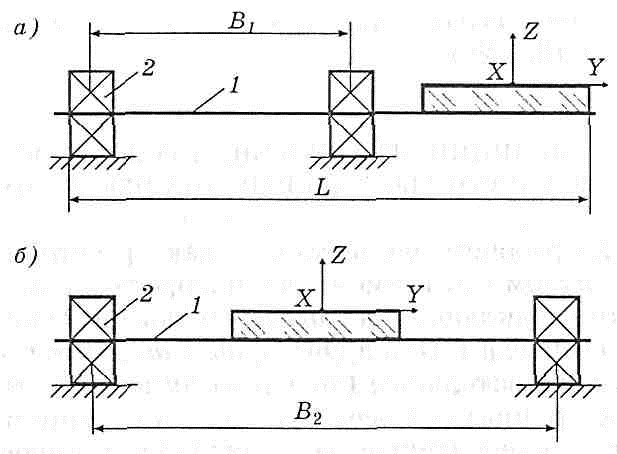
\includegraphics[width=0.6\textwidth]{4axe.png}
	\label{pic:4axe}
\end{figure}

\begin{flushleft}
\textbf{Принцип ограничения продольного и поперечного вылетов рабочих элементов}
\end{flushleft}

<<Вылетом>> рабочего элемента называют расстояние между ним и центром его возможного поворота в соединении. Суть принципа заключается в ограничении продольного или поперечного (иногда того и другого) вылетов, что позволяет уменьшить нежелательные (опасные) линейные смещения РЭС вдоль координатных осей при возникновении поворота рабочей детали относительно базовых элементов соединения из-за погрешностей формы сопрягаемых поверхностей, деформаций, зазоров.

Базирование оправы линзы (рис.~\ref{pic:4connlens}) в кронштейне, устанавливаемом на рейтере, приводит к тому, что узловая точка линзы (РЭС) имеет поперечный $ H $ и может иметь продольный $ L $ вылеты относительно возможного центра поворота оправы $ C $. В результате при повороте оправы на угол $ \Delta\gamma $  РЭС имеет смещение (расфокусировку) вдоль оси $ Z $ ( $ \Delta Z_{\Delta\gamma} \approx H\Delta\gamma$ ) и децентрировку вдоль оси $ X $ ( $ \Delta X_{\Delta\gamma} = L\Delta\gamma $ ). Штриховой линией на этом рисунке изображена конструкция кронштейна, позволяющая ограничить вылет $ L $.

\begin{figure}[h!]
	\caption{Сопряжение оправ линзовых систем с корпусной деталью}
	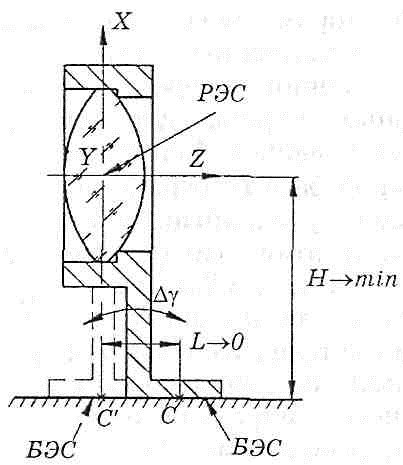
\includegraphics[width=0.4\textwidth]{4connlens.png}
	\label{pic:4connlens}
\end{figure}

\begin{flushleft}
\textbf{Учет тепловых свойств соединяемых деталей}
\end{flushleft}

Этот принцип заключается в обеспечении отсутствия возможных деформаций и смещений сопрягаемых деталей в соединении при отклонении температуры, от номинального значения.

Чаще всего указанные дефекты возникают из-за разности коэффициентов линейного расширения материалов базовой и присоединяемой деталей. Для соблюдения принципа следует обеспечить возможность относительного изменения размеров деталей (при отклонении температуры) без нарушения их взаимного базирования благодаря выбору соответствующих зазоров в посадке, упругому силовому замыканию, целенаправленному подбору материалов и размеров деталей, применяя термокомпенсаторы.

Рассмотрим типовое соединение линзы с оправой с помощью резьбового кольца (рис.~\ref{pic:4opt}~а).
\begin{figure}[H]
	\caption{Крепление оптических деталей в оправах}
	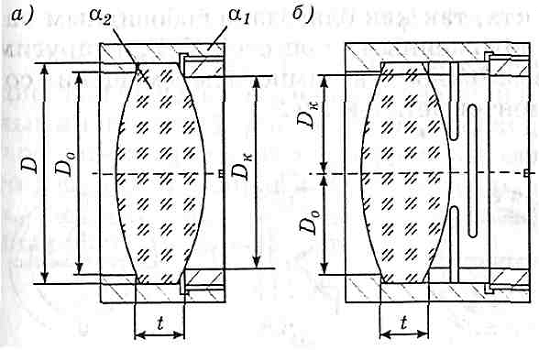
\includegraphics[width=0.6\textwidth]{4opt.png}
	\label{pic:4opt}
\end{figure}

Когда коэффициенты линейного расширения материалов оправы $ \alpha_1 $ и линзы $ \alpha_2 $ различны, отклонение температуры от номинального значения приводит к изменению диаметров $ D $ линзы и оправы, диаметров $ D_0, D_K $, размера $ t $. Это может вызвать либо деформацию линзы (и оправы), либо смещение линзы в зазоре. Например, когда посадка линзы в оправу по диаметру $ D $ обеспечивает необходимый температурный зазор, деформация или зазор возникают из-за несоответствия изменений $ D_0 $ и $ t $ линзы и оправы. Пружинное кольцо, помещенное между линзой и резьбовым кольцом (рис.~\ref{pic:4opt}~б), позволяет избежать указанных недостатков (при достаточном температурном зазоре в посадке), так как компенсирует осевое изменение размеров линзы и оправы, а также изменение диаметров $ D_0, D_K $.

\begin{flushleft}
\textbf{Точностная технологичность соединений}
\end{flushleft}

В процессе сборки детали соединяются путем сочленения, свинчивания, завальцовки или склейки.

Технологичность соединения определяется трудоемкостью сборки, трудоемкостью контроля качества сборки, уровнем необходимой квалификации персонала.
Наиболее технологичными являются соединения, которые могут быть собраны с использованием автоматического оборудования и промышленных роботов. Поэтому конструктор должен руководствоваться не только рассмотренными общими принципами конструирования соединений (выполнение которых, как правило, повышает их технологичность), но и частными правилами, касающимися автоматизации сборочных операций. Эти правила заключаются:
\begin{enumerate}
	\item в обеспечении полной взаимозаменяемости деталей;
	\item стремлении к симметрии относительно наибольшего числа осей;
	\item минимизации числа соединительных элементов;
	\item исключении одновременного начала контактирования сопрягаемых деталей по нескольким поверхностям;
	\item осуществлении центрирования с помощью вращательно-симметричных деталей;
	\item предотвращении кинематически сложного движения рабочей детали в положение для сборки с базовой.
\end{enumerate}

Одно из основных требований к качеству соединений~-- точность расположения их рабочих элементов относительно базовых (рис.~\ref{pic:4elements}). Оно достигается благодаря точному изготовлению соответствующих элементов сопрягаемых деталей, а также с помощью их доводок и регулировок (юстировок) в соединении. Получаемую при этом точность соединений можно отнести к группам пониженной, средней и высокой точности, которые по соответствующей трудоемкости их достижения называют часто экономическим, производственным, и техническим, уровнями точности сборки деталей.

\textit{Экономическому уровню} соответствует точность, достигаемая при сборке деталей без последующих пригонок и регулировок. Точность расположения рабочих элементов соединения относительно базовых при этом определяется погрешностями изготовления и сборки соответствующих элементов сопрягаемых деталей.

\textit{Производственному уровню} соответствует точность, достигаемая при сборке с применением пригонки, регулировки и универсального оборудования и инструмента, и контролем на качественном уровне либо простейшими контрольными и измерительными средствами (индикаторами, калибрами, уровнями, шаблонами).

Точность соединения тогда будет выше, так как часть погрешностей деталей компенсируется. Естественно, трудоемкость этой сборки будет выше.

\textit{Техническому уровню} соответствует точность, достигаемая при сборке с пригонками, регулировками и доводками и контроле с помощью прецизионных средств (автоколлиматоров, микроскопов, интерферометров), а также обеспечением соответствующих условий производства (стабилизации температуры, защиты от вибраций, чистоты рабочих мест).

\section{Принципы конструирования узлов и функциональных устройств ОЭП}

Узлы и функциональные устройства (ФУ) представляют собой более сложные, чем соединения, сборочные единицы, состоящие из большего числа деталей и элементов, которые могут выполнить совместно с другими составными частями ОЭП (или самостоятельно) определенную функцию. Это, например, объективы, окуляры, механизмы, сканирующие устройства, устройства крепления источников и приемников излучения, затворы, диафрагмы, столики, датчики. В узлах и ФУ целесообразно различать рабочие (исполнительные), базовые (несущие) и эталонные (образцовые) детали и рабочие (РЭУ), базовые (БЭУ) и эталонные (ЭЭУ) элементы устройств.

Основные показатели качества узлов и ФУ -- точность (расположения РЭУ относительно БЭУ и ЭЭУ) передачи и преобразования информации, качество создаваемого изображения, надежность и технологичность.

Рассматриваемые далее принципы заключаются в общих правилах конструирования механических и оптических ФУ прибора, позволяющих оптимизировать их структуру, внутренние связи и взаимодействие элементов в целях повышения упомянутых показателей качества создаваемых ФУ.

\begin{flushleft}
\textbf{Принцип АББЕ}
\end{flushleft}

По этому принципу, называемому также принципом исключения компараторной погрешности, эталонный элемент устройства должен быть расположен соосно с рабочим, элементом (или измеряемым объектом). В этом случае уменьшается погрешность взаимного линейного расположения эталонного и рабочего элементов при возникновении поворотов деталей из-за технологических или эксплуатационных погрешностей (зазоров, погрешностей формы контактирующих поверхностей, деформаций, биений).

На рис.~\ref{pic:4comparator} показан классический пример, давший второе название принципу с поперечным (рис.~\ref{pic:4comparator}~а) и продольным (рис.~\ref{pic:4comparator}~б) компараторами.
\begin{figure}[h!]
	\caption{Компараторы}
	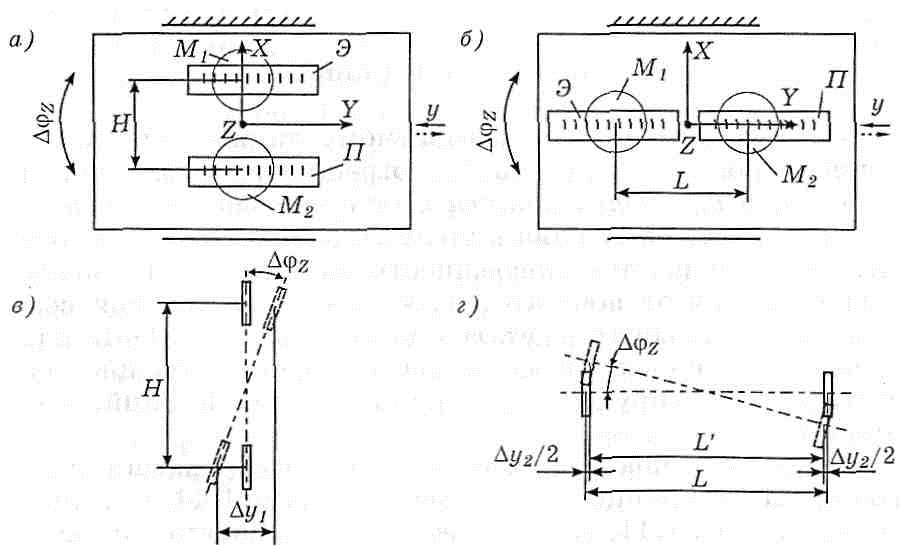
\includegraphics[width=1\textwidth]{4comparator.png}
	\label{pic:4comparator}
\end{figure}

На каретке, перемещаемой вдоль оси $ Y $, установлены эталонная Э и поверяемая П шкалы, взаимное положение штрихов которых измеряется с помощью отсчетных микроскопов $ M_1, M_2 $.

В поперечном компараторе, из-за поворотов каретки $ (\Delta \varphi_z) $ вокруг оси $ Z $, обусловленных погрешностями направляющих, возникает значительная погрешность измерения $ \Delta y_1 $ первого порядка малости, пропорциональная расстоянию $ Н $ между шкалами (рис.~\ref{pic:4comparator}~в):
\[ 
\Delta y_1 = H\,\sin\Delta\varphi_z\,\approx\, H\,\Delta\varphi_z
\]

Чтобы исключить погрешность первого порядка, Аббе предложил расположить эталонную и поверяемую шкалы соосно, преобразовав компаратор в продольный (компаратор Аббе). В этом случае погрешность измерения из-за поворотов каретки будет лишь второго порядка малости (рис.~\ref{pic:4comparator}~г):
\[ 
\Delta y_2 = L - L' = 2L\sin^2(\Delta\varphi/2) \approx L \Delta\varphi^2 /2.
\]

\begin{flushleft}
\textbf{Принцип кратчайшей цепи преобразования}
\end{flushleft}

Так же, как и кратчайшая размерная цепь (позволяющая получить более высокую точность размера замыкающего звена), кратчайшая цепь преобразования, содержащая минимальное число преобразователей, позволяет получить более высокую точность функционирования устройства благодаря меньшему числу источников погрешностей.

Сравним, например, теодолит и стереотрубу, функциональные схемы которых изображены на рис.~\ref{pic:4teodolit}.

\begin{figure}[h!]
	\caption{Функциональные схемы теодолита (а) и стереотрубы (б)}
	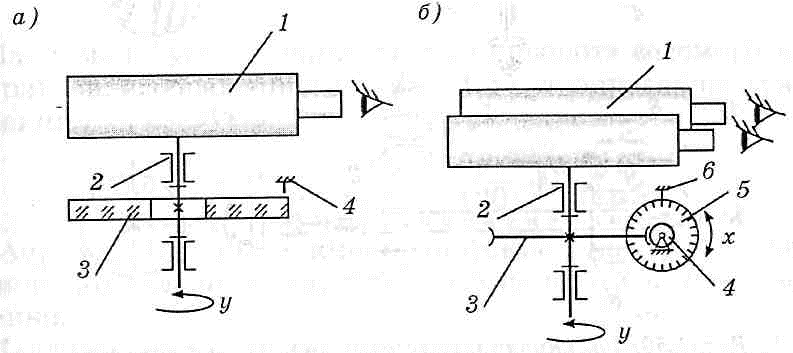
\includegraphics[width=1\textwidth]{4teodolit.png}
	\label{pic:4teodolit}
\end{figure}

Горизонтальные углы на местности измеряются теодолитом (рис.~\ref{pic:4teodolit}~а) при наведении зрительной трубы 1 на объект наблюдения (рейку) ее разворотом вокруг вертикальной оси 2 с помощью лимба 3 и индекса (отсчетной системы) 4. 

Измерения горизонтальных углов стереотрубой (рис.~\ref{pic:4teodolit}~б) осуществляются наведением зрительных труб 1 на объект их разворотом вокруг вертикальной оси 2 с помощью отсчетной червячной передачи 3, 4 и лимба 5 с индексом~6.

Теодолит, содержащий всего одну кинематическую пару (осевую систему), существенно превосходит по точности (погрешность измерения углов точными и грубыми теодолитами:  $ \Delta y=2\div30'' $) стереотрубу, кинематическая цепь которой содержит две осевые системы и отсчетную червячную передачу. 

Точность стереотруб не превосходит одной-двух минут и обуславливается главным образом кинематической погрешностью червячной передачи.

\begin{flushleft}
\textbf{Принцип наибольших масштабов преобразования}
\end{flushleft}

Согласно этому принципу функциональные элементы, осуществляющие наибольший масштаб преобразования, следует ставить в конце (для устройств, работающих на редукцию) либо в начале (для устройств, работающих на мультипликацию) цепи элементарных преобразователей, а также необходимо соотносить масштаб преобразования с погрешностями элементов. В этом случае суммарная погрешность устройства будет ниже.

\begin{figure}[H]
	\caption{Кинетические схемы, приводов}
	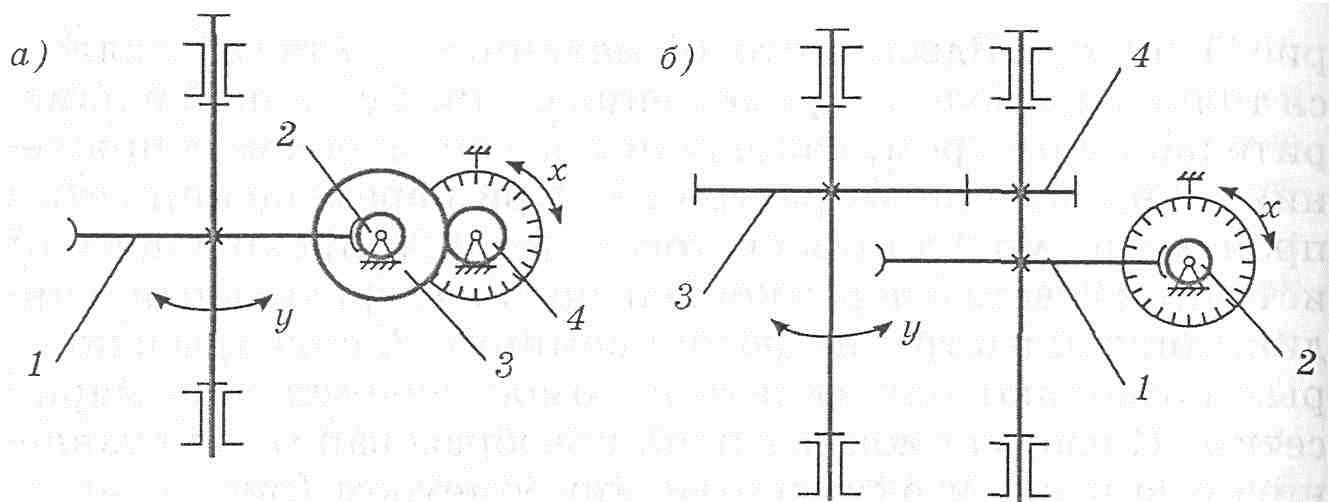
\includegraphics[width=1\textwidth]{4kinetic.png}
	\label{pic:4kinetic}
\end{figure}

На рис.~\ref{pic:4kinetic} показаны две схемы отсчетных приборов углоизмерительной бабки (стола). Оба привода состоят из одинаковых червячных 1, 2 и зубчатых 3, 4 пар, но переставленных местами. Червячные пары имеют передаточные отношения $ i_1 = 1 : 120 $, зубчатые $ i_2 = 1 : 3 $. Выходная координата у связана с входной х соотношением:
\[
y = i_1 \, i_2 \, x = \dfrac{1}{360}\,x. 
 \]

Максимальную погрешность угла поворота ведомого звена привода (рис.~\ref{pic:4kinetic}~а), определим из выражения:
\[ 
\Delta y_{max}^\text{а} = \Delta y_1 + \dfrac{\Delta y_2}{120}  + \dfrac{\Delta y_3}{120} + \dfrac{\Delta y_4}{360},
\]
где $ \Delta y_1 $, $ \Delta y_2 $, $ \Delta y_3 $, $ \Delta y_4 $ -- кинематические погрешности червячного колеса, червяка, зубчатого колеса 3 и 4 соответственно.

Максимальная погрешность другого привода (рис.~\ref{pic:4kinetic}~б) из-за этих причин
\[ 
\Delta y_{max}^\text{б} = \Delta y_3 + \dfrac{\Delta y_4}{3}  + \dfrac{\Delta y_1}{3} + \dfrac{\Delta y_2}{360}.
\]

Если для упрощения анализа примем, что  $ \Delta y_1 \approx \Delta y_2 \approx \Delta y_3 \approx \Delta y_4 $, получим
\[ 
\dfrac{\Delta y_{max}^\text{а}}{\Delta y_{max}^\text{б}} = \dfrac{1}{1,6}.
\]

Таким образом, привод, в котором элементарный преобразователь, имеющий наибольший масштаб преобразования, установлен в конце цепи преобразования, обладает точностью работы примерно в 1,6 раза выше, чем привод, где рассматриваемый принцип не выполняется.

\begin{flushleft}
\textbf{Принцип отсутствия избыточных связей и местных подвижностей в механизмах приборов}
\end{flushleft}

Избыточные связи в механизмах приборов приводят к объемным, деформациям звеньев, увеличению трения в кинематических парах, затрудняют сборку и регулировку механизмов. В результате ухудшается точность, надежность и технологичность сборки последних. Местные подвижности менее опасны, и обусловлены дополнительной рабочей подвижностью некоторых звеньев.

\begin{flushleft}
\textbf{Принцип необходимости юстировки оптических устройств}
\end{flushleft}

При конструировании оптических функциональных устройств следует проверять необходимость их юстировки и предусматривать в конструкции возможность ее выполнения.

\section{Общие принципы, правила и методы конструирования}

\begin{flushleft}
\textbf{Принцип унификации конструкций изделий}
\end{flushleft}

Унификацией называют приведение к оптимальному единообразию форм и объектов человеческой деятельности.
Что касается техники, то понятие унификации определяется согласно ГОСТ 23945.0-80 следующим образом: <<Унификация изделий -- приведение изделий к единообразию на основе установления рационального числа их разновидностей>>.

Суть принципа унификации конструкций изделий заключается в ограничении многообразия возможных частных (индивидуальных) решений на всех этапах проектно конструкторской деятельности рамками общих свойств и признаков, приводящих изделие к единой системе типовых конструкций.

\begin{flushleft}
\textbf{Компоновка конструкций}
\end{flushleft}

Компоновкой называют поиск и разработку рационального размещения элементов конструкции в заданном пространстве.

Именно в процессе компоновки создается конструкция будущего прибора, не только находится целесообразное взаимное расположение его модулей, устройств и узлов, но и определяются с учетом материалов оптимальные размеры и формы поверхностей деталей, отвечающие технико-экономическим требованиям задания и условиям производства. 
Так как от объема прибора зависит в известной степени его масса, занимаемая им площадь помещений, транспортные расходы, то общей тенденцией является стремление к уменьшению габаритных размеров конструкции при компоновке (т.е. к компактности конструкции).

При компоновке прибора, создаваемого при индивидуальном проектировании, также целесообразно разбивать прибор на функциональные составные части: несущие (базовые), преобразовательные (рабочие), коммуникационные (соединительные), вспомогательные.

Осуществляя компоновку, следует идти от общего к частному.

\textbf{Первый шаг.} В начале определяют, будет ли прибор моноблочным, когда все его составные части располагаются в одном корпусе, либо он будет состоять из нескольких самостоятельных частей (корпусов), связанных определенным образом друг с другом.

Решение этого вопроса зависит от назначения прибора, его характеристик, условий эксплуатации, уровня унификации, достижений и развития техники и других факторов.

\textbf{Второй шаг.} Заключается в эскизной компоновке общей конструкции моноблока (или автономного устройства) и его основных элементов без детализации принятого решения.

Эскизную компоновку следует начинать с решения вопроса, какой будет несущая (базовая) часть конструкции и каким способом будут сопрягаться с ней функциональные устройства (блоки) и элементы изделия. Например, несущей частью конструкции могут служить рама, стол, стойка, шкаф, шасси, штатив, кронштейн, труба, а функциональные блоки (модули), узлы и элементы могут устанавливаться путем выдвигания, нанизывания, накрытием.

Так как оптические приборы содержат функциональные устройства с различными физическими принципами действия (оптические, механические, электронные), которые должны располагаться в едином корпусе и быть защищены от внешних воздействий (посторонних засветок, механического контакта, загрязнений, влаги), то часто несущим элементом является коробчатый корпус, получаемый литьем из металлических или пластмассовых материалов.

Примерами могут служить хорошо известные всем конструкции фотоаппаратов, видеокамер.

\textbf{Третий шаг.} Определив несущую часть конструкции, продолжают эскизную компоновку узлов и основных деталей моноблока: оптических (объективы, призмы, растры), приводов (двигатели, зубчатые колеса, винтовые пары, рычаги, направляющие движения), источников и приемников излучения.

Второстепенные узлы, элементы и вспомогательные детали на этом этапе подробно могут не разрабатываться. Отдельные функциональные устройства, особенно унифицированные (электронные блоки, платы, редукторы, датчики), могут изображаться в конструкции в виде <<кубиков>>, сопрягаемых с несущими частями конструкции.

Удобнее всего компоновку вести в масштабе 1:1 (если объект конструирования не является сверхминиатюрным или, наоборот, слишком большим).

Одно из основных правил компоновки --- не останавливаться на одном (шаблонном или первом, пришедшим в голову) варианте конструкции, а попытаться разработать или отыскать несколько вариантов решения. Для дальнейшего анализа вариантов чаще всего достаточно иметь упрощенные их эскизы (наброски от руки), выполненные в одной-двух проекциях.

Всесторонний анализ найденных решений позволит выбрать наиболее рациональный и приступить к его детальной проработке и расчетам.

Залог успешной компоновки --- учет технологичности изготовления и сборки деталей; удобство юстировки, обслуживания и ремонта объекта конструирования.

При компоновке необходимо соблюдать 4 принципа:
\begin{enumerate}
	\item преемственности (ознакомиться с конструкцией с целью найти аналог);
	\item нужно действовать так точно, как необходимо и так просто, как доступно;
	\item повторное использование известных вариантов;
	\item новое качество может быть достигнуто не только с использованием принципиально новых решений, но и с помощью замены, добавления, изъятия, перестановки элементов. 
\end{enumerate}

Осуществляя компоновку, следует применять индивидуальный метод унификации конструкции, максимально используя стандартизованные, унифицированные и заимствованные из ранее спроектированных приборов функциональные устройства, узлы, детали и элементы. Это позволит ускорить конструирование, облегчить изготовление и повысить надежность. 

При этом также выполняется условие конструктивной преемственности -- использование предшествующего опыта оптической промышленности, точного приборостроения и машиностроения путем введения в разработку рациональных, проверенных на практике идей, конструктивных решений и технологий.

Осуществляя компоновку конструкций, целесообразно:
\begin{enumerate}
	\item исключать возможное вредное влияние отдельных функциональных устройств и элементов на другие (вследствие вибраций, температурного излучения, нагрузок);
	\item производить рациональное членение конструкций на составные части (функциональные устройства, узлы), обеспечивающие параллельность сборки и независимость юстировки и контроля;
	\item сочетать компактность конструкции с удобствами сборки, юстировки, технического обслуживания и ремонта ОП и его узлов в процессе изготовления и эксплуатации прибора;
	\item шире использовать принцип конструктивной инверсиии совмещения функций элементов ОП;
	\item используя в качестве компоновочных элементов зеркально-призменные системы, располагать их, по возможности, в параллельном ходе лучей с небольшими апертурами; не «разрывать» компоновочным элементом автономную функциональную систему (например, объектив, окуляр).
\end{enumerate}

В зависимости от назначения и от условий работы ОЭП применяются следующие компоновочные схемы (КС):
\begin{itemize}
	\item децентрализованную (разбросанную);
	\item полностью централизованную;
	\item централизованную с автономным пультом управления.
\end{itemize}

При децентрализованной КС каждый из блоков прибора конструируется отдельно и размещается автономно, а функционирование системы обеспечивается системой соединительных кабелей. Данную схему применяют, когда ОЭП служит для измерения параметров чего-либо без доступа оператора (например, для измерения ширины горячего проката стали: оптический блок ставят непосредственно на горячем стане вблизи контролируемого объекта, т.е. в неблагоприятных температурных условиях; электронный блок и блок питания недалеко, в более щадящих условиях, а блок индикации и регистрации -- в кабине оператора).

Децентрализованную схему компоновки часто используют в полевых приборах, что связано с транспортированием и ограничением массы; например, портативный тепловизор (устройство для наблюдения за распределением температуры исследуемой поверхности -- цветная картинка), состоящий из: оптического блока, электронного блока с пультом управления и индикации, соединительных кабелей и блока питания.

Достоинствами децентрализованной схемы являются простота компоновки отдельных функциональных блоков, возможность их произвольного размещения, достаточно высокая надежность, связанная с быстрой заменой вышедших из строя блоков простым переключением соединительных кабелей.
 
Недостатками рассматриваемой схемы являются наличие соединительных кабелей значительной длины, необходимость обеспечения индивидуальной защиты от вредных воздействий (температуры, влажности, вибраций) каждого функционального блока.

При полностью централизованной схеме компоновки все блоки размещаются в общем корпусе. Такая схема характерна для стационарно устанавливаемых приборов и широко используется в оптико-электронном приборостроении. По этой схеме выполнены многие лабораторные приборы: фотометры (для измерения фотоэлектрических световых величин), спектрометры, гониометры (прибор для измерения углов между плоскими гранями, измерение показателей преломления и дисперсии прозрачных твердых тел). По этой схеме строят приборы астроориентации, космических исследований, технологическое оборудование с использованием лазеров, контрольно-измерительные приборы.

Иногда компоновку выполняют по централизованной схеме с автономным пультом управления. Например, фотоэлектрическое устройство для дистанционного задания и измерения угла поворота объекта, в котором фотоэлектрический датчик, привод, электронный блок, блок питания скомпонованы в общем корпусе, установленном на объекте, а пульт управления и индикации вынесен в зону размещения оператора. Возможен также вариант с автономным оптическим блоком и централизованной компоновкой остальных блоков прибора.

Достоинствами централизованной схемы являются компактность прибора, минимальная длина междублочных связей, возможность обеспечения одновременной защиты всех блоков от внешних воздействий. 
К недостаткам этой схемы следует отнести возможность взаимного влияния отдельных блоков или элементов и сложность транспортирования, если габаритные размеры и масса прибора получаются большими.

Независимо от выбранной компоновочной схемы при конструировании прибора необходимо учитывать следующие общие принципы:
\begin{itemize}
	\item Конструкцию необходимо делить на узлы по функциональному признаку.
	\item Узлы и блоки прибора по возможности должны быть законченными с точки зрения производства и не требовать после сборки дополнительной обработки совместно с другими частями, позволять автономную проверку качества их функционирования.
	\item Конструкция должна обеспечивать возможность сборки как отдельных узлов, так и прибора в целом.
	\item Число деталей, входящих в сборку, должно быть по возможности наименьшим.
	\item Элементы и блоки необходимо устанавливать так, чтобы они не препятствовали прохождению лучей.
	\item Необходимо согласовывать движения перемещающихся частей прибора таким образом, чтобы исключить их столкновение и попадание в ход лучей.
	\item При монтаже в общем кожухе отдельные узлы и блоки во время работы не должны оказывать вредного взаимного воздействия (влияния теплового излучения, бликов, наводок, вибраций).
	\item В условиях эксплуатации прибора необходимо предусмотреть возможность быстрой замены отдельных элементов или блоков.
	\item Конструкция деталей, входящих в сборку, должна быть технологичной. Для деталей серийного и массового производства необходимо стремиться к сокращению механической обработки резанием. Корпусные детали и детали сложной формы следует изготовлять, используя точное литье, штамповку и другие методы обработки без снятия стружки. Для деталей единичного и мелкосерийного производства применение литья или штамповки экономически нецелесообразно. Сложные и корпусные детали рационально изготовлять из отдельных элементов, соединяя их сваркой, клепкой, сборкой на винтах.
	\item При компоновке следует учитывать требования по герметизации, термостатированию, экранированию, а также требования к конструкции, определяемые условиями эксплуатации и размещения прибора.
\end{itemize}

В настоящее время не существует какой-либо общей методики выполнения компоновки ОЭП. Конструирование и компоновку приборов выполняют в каждом конкретном случае индивидуально.

Для облегчения процесса компоновки часто выполняют оптико-кинематическую схему. Наряду с этим при конструировании узлов и компоновке прибора в целом необходимо предусматривать возможность последующей сборки, юстировки и контроля параметров. При сборке и юстировке отдельных узлов и прибора в целом конструкция их должна позволять проводить предусмотренные методикой юстировки подвижки и развороты оптических деталей или систем деталей. Поэтому при составлении методики юстировки должно быть определено, какие детали и в каких пределах могут перемещаться или разворачиваться для обеспечения требуемых технических характеристик и качества изображения. При этом следует стремиться к тому, чтобы каждая оптическая деталь при юстировке имела только одно перемещение.

\begin{flushleft}
	\textbf{Компоновка оптико-механических блоков}
\end{flushleft}

Рассмотрение различных конструкций ОЭП свидетельствует о том, что независимо от принятой компоновочной схемы можно выделить следующие основные способы компоновки прибора в целом или отдельных его блоков:
\begin{enumerate}
	\item В едином корпусе Характерна для приборов относительно небольших размеров, когда необходимо добиться их компактности и высокой жесткости. При массовом или крупносерийном способе производства корпусные детали изготовляют обычно методами точного литья, а при единичном и мелкосерийном -- на универсальном оборудовании. В соответствии с этим и должны быть сконструированы корпусные детали.
	
	\item С применением трубы в качестве несущего элемента. Конструкция фотоэлектрического автоколлиматора. Достоинством этого способа компоновки являются высокая жесткость и стабильность конструкции, поэтому его широко используют при создании контрольно-юстировочной аппаратуры, высокоточных угломерных устройств.
	
	\item С помощью рамы, выполненной из труб, угольников и других профилей. Этот способ компоновки может быть рекомендован для приборов и стендов, имеющих значительные габаритные размеры. Кроме того, его часто применяют на этапе макетирования. Достоинством такой компоновки является простота изготовления несущей конструкции и монтажа узлов, их доступность при настройке и юстировке. Недостатком компоновки с помощью рамы может быть нестабильность конструкции, особенно при изготовлении ее с помощью сварки. По этой же причине следует избегать сложных каркасов и стремиться к симметрии их конфигурации. Для повышения жесткости и стабильности в конструкцию рамы можно вводить косынки (пластины, связывающие звенья каркаса вблизи узлов соединения). Длина ребер рамы должна быть подобрана или рассчитана таким образом, чтобы при изменении температурного режима не происходило недопустимых деформаций рамы в целом или отдельных ее участков.
	
	\item На монтажной плите. Способ компоновки на монтажной плите применяют при конструировании приборов высокой стабильности, оптические элементы которых должны располагаться в одной плоскости. Все элементы устанавливаются на кронштейнах и стойках на единую плиту. Такой способ компоновки часто применяют для приборов, имеющих небольшие габаритные размеры, а также для соединения отдельных узлов в группы при использовании, например, рамной системы. Пример такой компоновки показан на рис.~\ref{pic:4LaserShow}~и \ref{pic:4LaserShow}.
	
	\begin{figure}[h!]
		\caption{ Пример компоновки на монтажной плите интерферометра Маха-Цендера }
		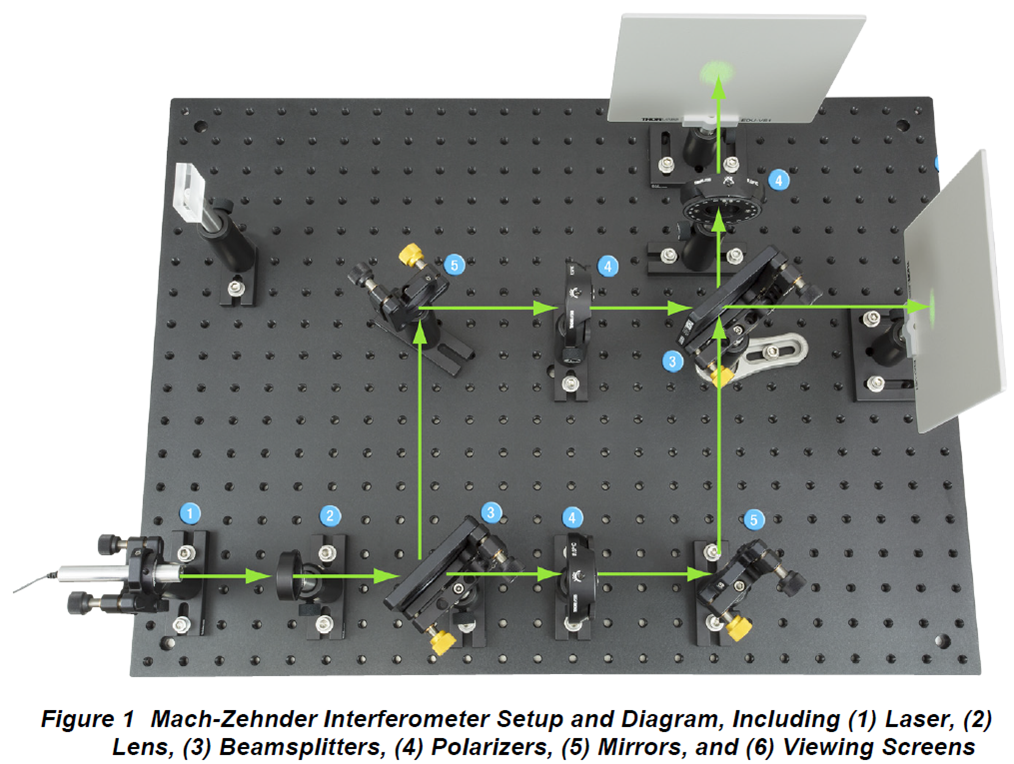
\includegraphics[width=0.9\textwidth]{4Montage.png}
		\label{pic:4Montage}
	\end{figure}
	
	\begin{figure}[h!]
		\caption{ Пример компоновки на монтажной плите проектора для лазерного шоу компании Arctos }
		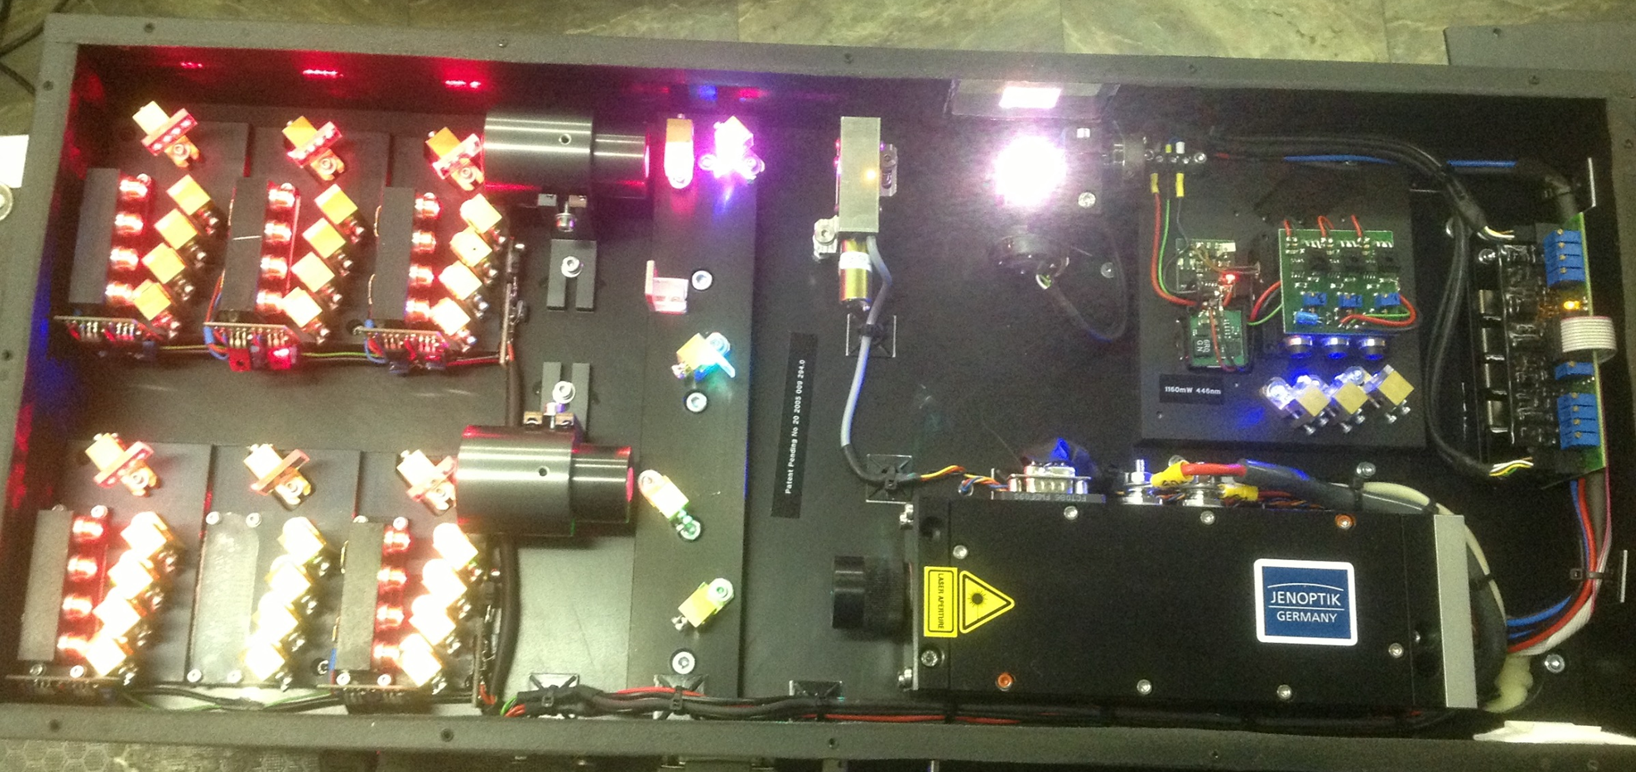
\includegraphics[width=0.9\textwidth]{4LaserShow.png}
		\label{pic:4LaserShow}
	\end{figure}
	
	\item На монтажных платах с колонками. Способ компоновки на монтажных платах с колонками является развитием предыдущего способа при расположении элементов оптической схемы в разных плоскостях. Как видно на рис.~\ref{pic:4plata}, в конструкцию прибора включены три монтажные платы~1, соединенные между собой колонками~2. На двух верхних платах в оправах, на стойках и кронштейнах размещены оптические элементы, а на нижней плате закреплен блок усилителей.
	
	\begin{figure}[h!]
		\caption{Компоновка на монтажных платах с колонками}
		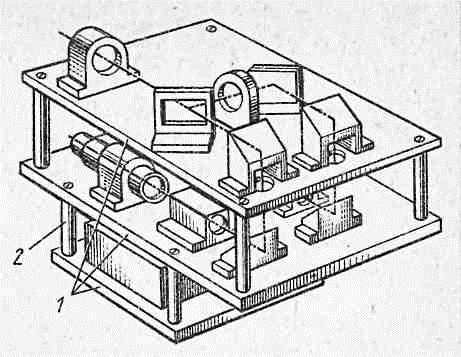
\includegraphics[width=0.9\textwidth]{4plata.png}
		\label{pic:4plata}
	\end{figure}
	
	\item С нанизыванием узлов. Компоновку с нанизыванием узлов применяют, если узлы прибора собраны на платах, имеющих одинаковую конфигурацию. Так, узлы объектива 1, светоделителя 2, модулятора 3, конденсоров 4, приемников излучения 5 и электронный блок 6 фазового угломера (рис.~\ref{pic:4uzel}~и \ref{pic:4uzel}) смонтированы на пластинах круглой формы, нанизанных на систему из трех стержней~7.
	
	\begin{figure}[h!]
		\caption{Компоновка с нанизыванием узлов}
		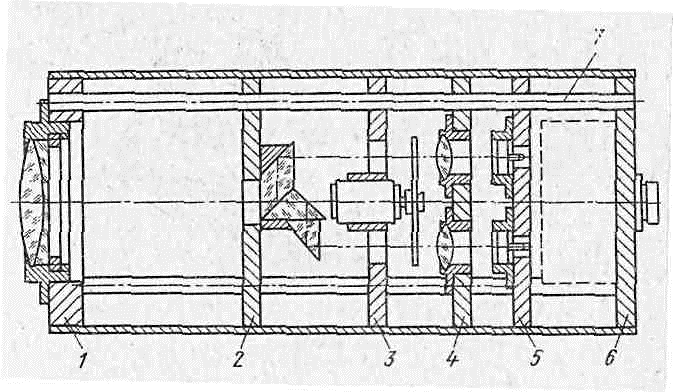
\includegraphics[width=1\textwidth]{4uzel.png}
		\label{pic:4uzel}
	\end{figure}
	
	\begin{figure}[h!]
		\caption{Компоновка с нанизыванием узлов компании Thorlabs}
		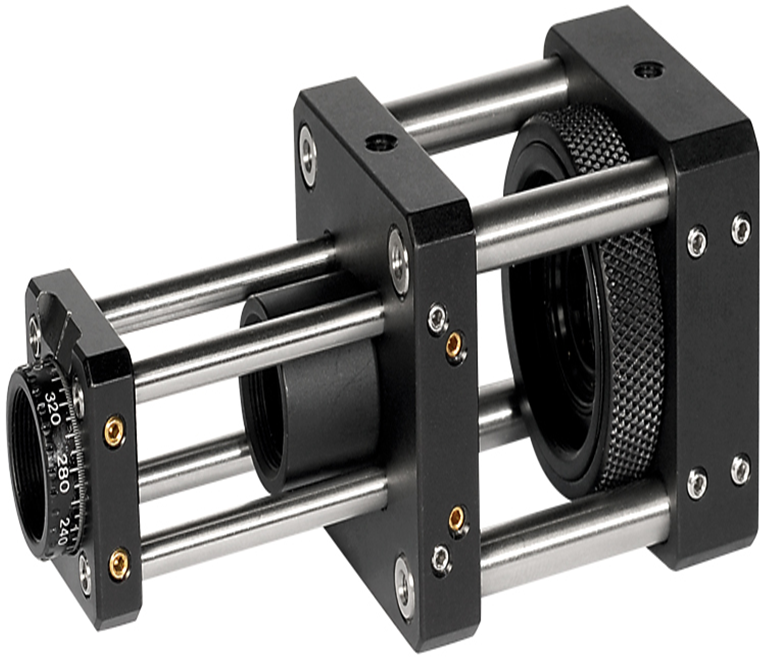
\includegraphics[width=0.7\textwidth]{4Nanizivanie.png}
		\label{pic:4Nanizivanie}
	\end{figure}
	
	Достоинством этой схемы компоновки являются единообразие несущих элементов, простота сборки и юстировки. Жесткость и стабильность такой конструкции не намного ниже аналогичных параметров конструкции при компоновке с применением трубы в качестве несущего элемента, а масса прибора значительно меньше. Поэтому компоновку с нанизыванием узлов часто применяют при конструировании крупногабаритных приборов, которые имеют осесимметричную схему и к которым предъявляют повышенные требования относительно жесткости.
	
	\item С использованием направляющей. Компоновка с использованием направляющей применяется при проектировании приборов, в которых при эксплуатации требуется изменять взаимное положение элементов (изменять расстояние между элементами, менять их местами) В основном это относится к стендовому оборудованию или приборам для научных исследований. В качестве примера такой компоновки можно привести оптическую скамью ОСК-2. Подобного рода компоновку выполняют также на направляющей треугольного профиля.Направляющая типа <<Ласточкин хвост>> показана на рис.~\ref{pic:4Lastochkin}.
	
	\begin{figure}[h!]
		\caption{Компоновка на монтажных платах с колонками}
		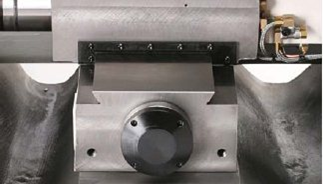
\includegraphics[width=0.5\textwidth]{4Lastochkin.png}
		\label{pic:4Lastochkin}
	\end{figure}
	
	\item В стойку с использованием модульных узлов и блоков. Компоновку на базе модульных узлов и блоков применяют в основном при конструировании электронных стоек.
	
	\item В кожух в виде пульта.
\end{enumerate}

Способы компоновки 3-8 в большинстве случаев требуют применения кожуха, защищающего прибор от посторонних засветок и воздействия окружающей среды. Во многих случаях при конструировании оптических блоков ОЭП используют одновременно несколько рассмотренных способов компоновки

\begin{flushleft}
	\textbf{Некоторые примеры компоновки}
\end{flushleft}

Так как ОЭП содержат функциональные устройства с различными физическими принципами действия (оптические, механические, электронные), которые должны располагаться в едином корпусе и быть защищены от внешних воздействий (посторонних засветок, механического контакта, загрязнений, влаги), то часто несущим элементом является коробчатый корпус, получаемый литьем из металлических или пластмассовых материалов.

Командно-регистрационные устройства ОЭП выполняются, как правило, в виде автономных блоков по принципу блочно-модульной конструкции. На рис.~\ref{pic:4block} изображен подобный автономный блок с несущим элементом -- стойкой, в которую вдвигаются функциональные блоки (модули) 1-7. На рис.~\ref{pic:4NI} показана компоновка модульной PXI-платформы компании National Instruments.

\begin{figure}[H]
	\caption{Компоновка командно-регистрационного устройства}
	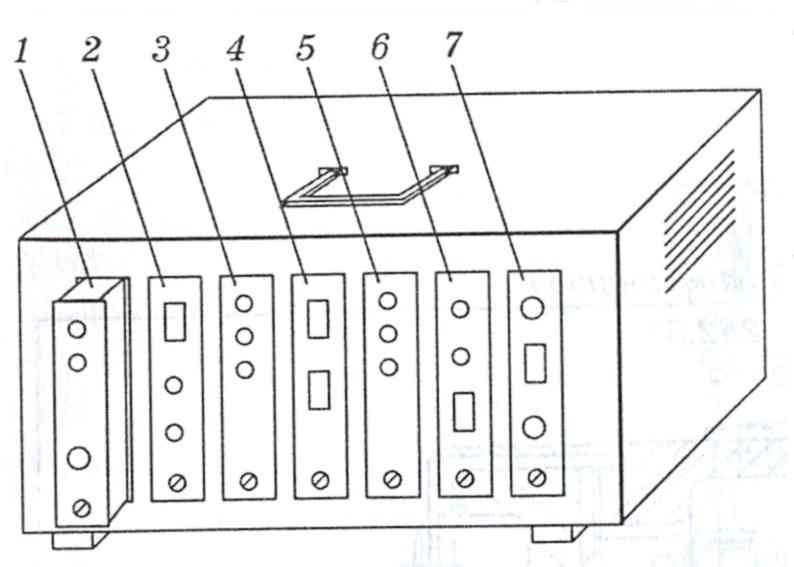
\includegraphics[width=0.6\textwidth]{4block.png}
	\label{pic:4block}
\end{figure}

\begin{figure}[H]
	\caption{ Компоновка модульной PXI-платформы компании National Instruments }
	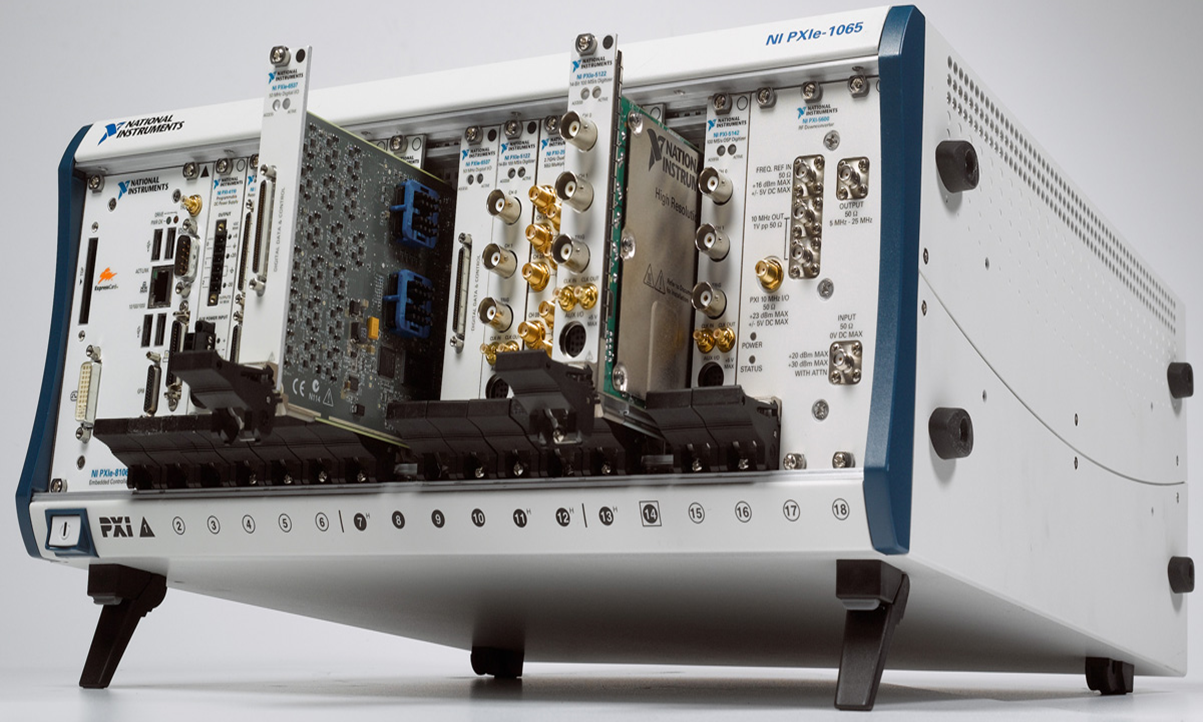
\includegraphics[width=0.8\textwidth]{4NI.png}
	\label{pic:4NI}
\end{figure}

Компонуя оптическую схему прибора, часто используют зеркально-призменные системы (ЗПС). При этом целесообразно учитывать свойства этих систем, позволяющие упростить юстировку при сборке и выполнить конструкцию более устойчивой к разъюстировкам в процессе эксплуатации.

На рис.~\ref{pic:4prism}, а показана схема компоновки объектива~1 и фотоприемника~3 с помощью прямоугольной призмы~2. Для центрировки и фокусировки изображения на фотоприемник призму юстируют. Если сместить ее по оси $ Z $ (или в другом произвольном направлении), то появляется смещение изображения по приемнику вдоль оси $ X' $ и вдоль оси $ Z' $, т.е. юстировка является зависимой. Кроме этого, при такой подвижке возможны повороты призмы вокруг оси $ Y $, которые вызовут смещение и наклон изображения.

Компоновка конструкции с помощью пентапризмы (рис.~\ref{pic:4prism}~б) более предпочтительна, так как, сдвигая ее вдоль оси $ X $, добиваются центрировки изображения (его смещения вдоль оси $ X' $), а сдвигом вдоль оси $ Z $ -- юстировка будет менее трудоемкой, так как является независимой.

\begin{figure}[h!]
	\caption{Компоновки конструкции призмами}
	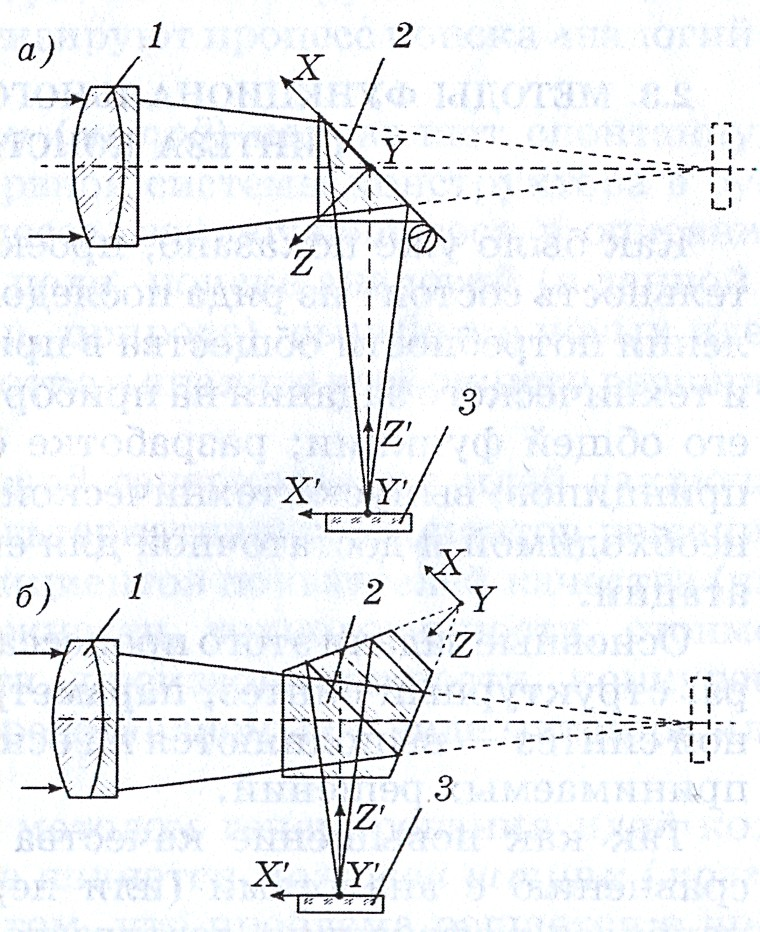
\includegraphics[width=0.7\textwidth]{4prism.png}
	\label{pic:4prism}
\end{figure}

Еще один пример компоновки с использованием принципа инверсии (Под конструктивной инверсией понимают перестановку, обращение или перераспределение роли и функций деталей, узлов, их элементов для улучшения свойств конструкции без изменения ее общей целевой функции) для упрощения конструкции корпуса телеобъектива показан на рис.~\ref{pic:4inversion}. В первоначальном варианте (рис.~\ref{pic:4inversion}~а) изменение воздушного промежутка $ d $ между подвижным положительным~2 и неподвижным отрицательным~3 компонентами телеобъектива достигалось вращением оправы положительного компонента, сопрягаемого с корпусом по резьбе. Так как диаметр оправы компонента~2 и диаметр компонента~3 существенно различаются, конструкция корпуса~1 получилась сложной и нетехнологичной.

Второй вариант конструкции телеобъектива (рис.~\ref{pic:4inversion}~б), где перемещается по резьбе оправа~4 отрицательного компонента (относительно неподвижного положительного), позволяет упростить конструкцию корпуса~5, создает возможность изготовить его из стандартной трубы, сократить расход материала.

\begin{figure}[h!]
	\caption{Конструктивная инверсия элементов объектива}
	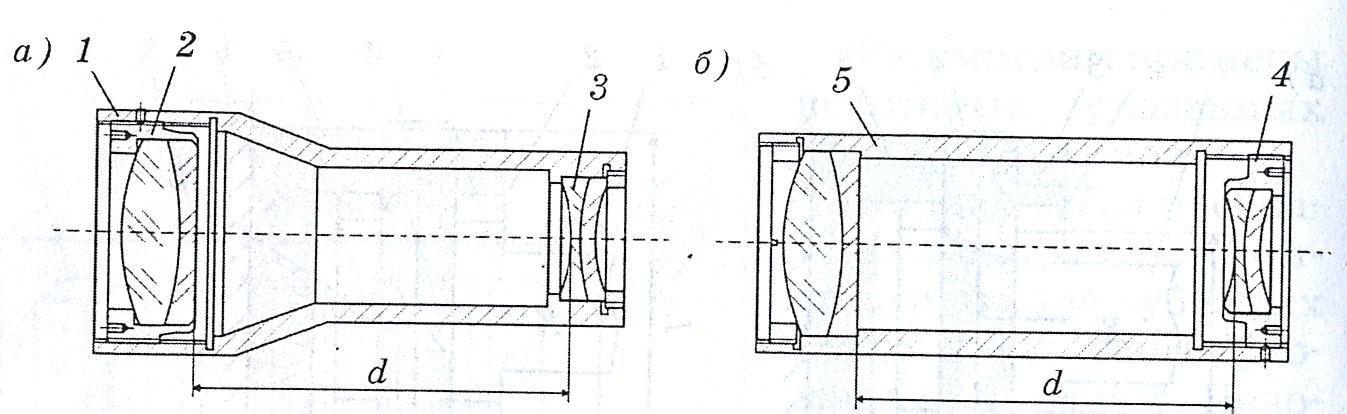
\includegraphics[width=1\textwidth]{4inversion.png}
	\label{pic:4inversion}
\end{figure}
